%\documentclass[12pt,letterpaper]{article}

%\usepackage[dvips]{graphicx}

%\begin{document}

%\begin{center}
%{\LARGE DESCRIPTION OF CTRAJ}
%\end{center}

%\tableofcontents

\subsection{Basic algorithm}

The only thing that CTRAJ does is integrate 
the following pair of ordinary differential equations:
\begin{equation}
\frac{\mathrm d \vec x}{\mathrm d t} = \vec v(\vec x, ~t)
\end{equation}
where $\vec x=(x, y)$ is position, 
$t$ is time
and $\vec v = (u, v)$ is a known velocity field.
We term this the ``trajectory equation.''
All other codes are built up from this base.
The codes take a set of initial points (which we will call the initial "field")
and integrates them forward in time.
The velocity field is gridded in a Cartesian space and linearly interpoled.
The trajectory equation is integrated
using a Runge Kutta fourth order method with constant step size.

\subsection{Transformed coordinates}

The codes are general enough that any velocity field can
be integrated, so long as it is gridded in a Cartesian space.
Since the velocities are encapsulated in container classes,
adaptation to a non-gridded format or analytical computation
of velocities will be quite straightforward.
However the main purpose of these codes is to advect velocities
over the surface of the Earth (e.g. output from GCMS, assimilation data,
etc.) thus they must be transformed to a suitable projection.
We use an azimuthal equidistant projection limited to one hemisphere.
This has the dual advantage of eliminating the singularity at the
pole and having relatively little variation in the area of each grid cell.

The transformations from standard longitude-latitude 
(constant diameter spherical polar) coodinates are as follows:
\begin{eqnarray}
x & = & r \cos \theta \\
y & = & r \sin \theta
\end{eqnarray}
where $r$ is defined as follows:
\begin{equation}
r = \sqrt{x^2 + y^2} = R (\pi/2 - h \phi)
\end{equation}
where $\theta$ is longitude in radians,
$\phi$ is latitude in radians,
$R$ is the radius of the Earth
and $h$ is the pole upon which the transformation is centred:
\begin{equation}
h = \left \lbrace \begin{array}{rl} 1; & \mathrm{North} \\ -1; & \mathrm{South} \end{array} \right .
\end{equation}
The resulting space has the following metric:
\begin{eqnarray}
\left (\frac{ds}{d x} \right )^2 & = & \frac{1}{r^2} \left [
	\frac{R^2}{r^2} \sin^2 \left (\frac{r}{R} \right ) 
	y^2 + x^2 \right ] \\
\left (\frac{ds}{d y} \right )^2 & = & \frac{1}{r^2} \left [
	\frac{R^2}{r^2} \sin^2 \left (\frac{r}{R} \right )
	x^2 + y^2 \right ]
\end{eqnarray}
while the reverse transformations are given as:
\begin{eqnarray}
\phi & = & h \left ( \frac{\pi}{2} - \frac{r}{R} \right ) \\
\theta & = & \tan^{-1} \left (\frac{y}{x} \right )
\end{eqnarray}

\begin{center}
\includegraphics[width=0.8\textwidth]{grid_example.ps}
\end{center}

The velocity field transforms as follows:
\begin{eqnarray}
\frac{\mathrm d x}{\mathrm d t} & = & - h v \frac{x}{r} - 
		\frac{u y}{R \sin (r/R_e)} \\
\frac{\mathrm d y}{\mathrm d t} & = & - h u \frac{x}{r} - 
		\frac{v y}{R \sin (r/R)}
\end{eqnarray}
where $u$ is the zonal wind and $v$ is the meridional wind.
To run the simulation over the entire surface of the Earth
we use two fields, one for the Northern hemisphere and one for the Southern.
These fit together like two halves of an eggshell.
Since equatorial crossings are relatively rare, 
we only check for them at intervals (typical when the field is output).
For this reason, the velocity fields overlap slightly, as seen in the figure.
The following transformations convert a coordinate to its equivalent
representation in the opposite hemisphere:
\begin{eqnarray}
r_{-h} & = & \pi R - r_h \\
x_{-h} & = & \frac {r_{-h} } 
	{r_h} x_h \\
y_{-h} & = & \frac {r_{-h} } 
	{r_h} y_h
\end{eqnarray}
Where the subscript $h$ labels the hemisphere.

\begin{center}
\includegraphics[width=0.6\textwidth]{tracer_coord.ps}
\end{center}

\subsection{Contour advection}

Consider a blob of dye stirred by a moving fluid.
To first order it can modelled by tracing its outlines
and allowing these to move with the fluid.
Contour advection is an adaptive method of modelling the
contours or isolines of a passive tracer.
It works by following the trajectories from points at intervals along
the contour.  
To maintain the integrity of the curve,
new points are added or removed as needed.

We want the points to lie at roughly constant intervals
along the curve even as it is stretched in many directions
at once.
Rather than use intervals of constant distance, we use fraction of arc:
\begin{equation}
c \Delta s \approx const.
\end{equation}
where $c$ is the radius of curvature and for a Cartesian
space is calculated as follows:
\begin{equation}
\frac{1}{c^2} = \left ( \frac{\partial x}{\partial s} \right )^2 +
		\left ( \frac{\partial y}{\partial s} \right )^2
\end{equation}
The path along the curve, $s$, is first approximated as a set of piece-wise
continous line segments.
The resulting parametric representation of the contour
is interpolated using a cubic spline.
A cubic spline returns a set of second-order
derivatives with which we can calculate the curvature:

New points are added between pairs of points that trace
out either too large an arc or too great a distance.
Likewise, points are removed if they are too close to their neighbour.

\subsection{Semi-Lagrangian advection}

A passive tracer simulation aims to solve the following
differential equation, termed the advection equation:
\begin{equation}
\frac{\mathrm d q(\vec x_0,~t)}{\mathrm d t}=S
\end{equation}
where $q$ is the tracer field in Lagrangian space, $\vec x_0$
and $S$ is the source term.
While $S$ can accomodate other sources,
such as chemical rates, here we concern ourselves with
the diffusion term:
\begin{equation}
S = \nabla \left [ D \nabla q(\vec x,~t) \right ]
\end{equation}
where $D$ is the diffusivity tensor.
In an Eulerian framework, this becomes:
\begin{equation}
\frac{\partial q(\vec x,~t)}{\partial t} + \vec v(\vec x,~t) \cdot \nabla q(\vec x,~t) = \nabla \left [ D \nabla q(\vec x,~t) \right ]
\end{equation}

\includegraphics[width=0.8\textwidth]{semi_Lagrangian.ps}

Since, in the absence of diffusion, tracer values are constant
along the trajectories, we can build a tracer simulation
using only the trajectory integrator.
The idea is to define an Eulerian grid and 
run back-trajectories from each grid point.
Values of the tracer for the current field are
interpolated from the previous field.

Because it doesn't matter in what order the trajectories 
are run (they are independent of the tracer field)
and because the interpolation defines a series of coefficients
mapping a tracer field from one time step to the next,
we write these coefficients into a sparse matrix.
The sparse matrix will have sides the size of
the number of tracer grid points.
A mapping from a two-dimensional tracer field
to a one-dimensional vector must be defined.

Expressing this mathematically:
\begin{equation}
\vec q (t_i) = A_{i} \cdot \vec q(t_{i-1})
\end{equation}
where $\vec q(t_i)$ is the tracer field at the $i$th
timestep and $A_i$ is a matrix.

A semi-Lagrangian simulation is not subject to the CFL criterion
and is unconditionally stable.
 The interpolation step provides a small amount of diffusion,
thus to essentially eliminate it, we make the Eulerian time step
(that controls the interpolation between fields) the same
size as the total integration time.

\subsection{Efficiency}

The advection codes spend the majority of their time
interpolating the velocity field.
We have mitigated this in the case of the tracer simulation
by writing coefficients to an array of sparse matrices
thus the tracer simulation needs only be run once over a given
period of time.

\subsection*{References}

\begin{itemize}

\item{D. G. Dritschel (1988). "Contour surgery: A topological reconnection scheme
for extended integrations using contour dynamics." {\it Journal of
Computational Physics} 77, 240-266.}
\item{W. H. Press, S. A. Teukolsky, W. T. Vetterling, B. P. Flannery, B. P. (1992).
{\it Numerical Recipes in C, 2nd Edition.} Cambridge University Press,
Cambridge, UK.}
\end{itemize}

%\end{document}



